\documentclass[a4paper, 12pt]{article}

\usepackage[utf8]{inputenc}
\usepackage{graphicx}
\usepackage{amsmath}
\usepackage{amsfonts}
\usepackage{amssymb}
\usepackage{hyperref}
\usepackage{geometry}
\usepackage{natbib}
\geometry{a4paper, margin=1in}

\title{Evolutionary Dynamics and Adaptation}
\author{Krishna Vadali\\
        \textit{Institute for Computing in Research} \\
        \textit{krishnavvk07@gmail.com}}
\date{\today}

\begin{document}

\maketitle

\begin{abstract}
Your abstract goes here. It should be a brief summary of the This study investigates the impact of the Yersinia Pestis bacteria in altering genes, while potentially offering selective immunity over the Black Death. Through extrapolation of data and analysis of plotting results, it was found that a protective allele A/A of the single nucleotide polymorphism (SNP) rs2549782 within the ERAP2 gene offered selective immunity during the Black Death. However, it was also found that it subsequently found that having the protective genotype variation also might be associated with an increase in risk of autoimmune disorders. Historical data was analyzed to assess how this genotype of the SNP rs2549782 has evolved and its protective allele frequencies in modern days reveal a strong presence in the region of interest. Our findings reveal that this SNP conferred a relative immunity to the disease, suggesting a survival advantage during the epidemic. However, this same genetic variant is linked to an increased risk of autoimmune disorders in latter populations. 
\end{abstract}

\section{Introduction}
The Black Death, one of the most devastating pandemics in human history, swept through Europe in the mid-14th century, profoundly impacting society, economy, and culture. Originating in Central Asia, likely from the steppes of Mongolia, the plague bacterium Yersinia pestis spread rapidly through trade routes, arriving in Europe in 1347 and killing an estimated 25 to 30 million people. 

This catastrophic event not only caused immense human suffering but also led to significant social, economic, and cultural changes, reshaping the medieval world. In this context, the role of genetic factors, such as the Endoplasmic Reticulum Aminopeptidase 2 (ERAP2) gene, becomes crucial. ERAP2 is involved in the immune system by processing antigenic peptides for paper by MHC class I molecules, thus influencing an individual's immune response. Single nucleotide polymorphisms (SNPs) like rs2549794 in ERAP2 can affect disease susceptibility and immune efficiency.

This paper investigates the allele frequencies of rs2549794 in historical and modern populations to explore its association with immunity against the Black Death and its potential link to increased susceptibility to autoimmune disorders. By examining these genetic variations, an understanding can be reached as to how the Black Death influenced genetic selection and how protective genetic factors against historical pandemics may have implications for modern disease susceptibility.

\section{Literature Review}
Most of the research conducted on relationships between pathogens and genes, such as the Y. Pestis and ERAP2 gene, focuses solely on how one factor affect the other. However, it is worth researching how these relationships translate into modern-day genomics, and whether the observed trends during the history of the gene have carried over to the modern age.

\section{Methodology}
\subsection{Data Collection}
The sequencing data for the ERAP2 gene during the time of the Black Death and its SNPs was imported from the NCBI database. The datasets for allele frequencies, FST values, and cytokine values were collected and processed to better suit the nature of the project. The modern-day allele frequencies and population data were retrieved from The Allele Frequency Database.

\subsection{Data Filtration}
To make sure that a proper study is conducted on the role of Y. Pestis bacteria in causing autoimmune disorders, the first step was to find commonality between the two entities, which in this case is the presence of SNPs based on how often their alleles occur in the population of London pre, during, and post Black Death.

Next, based on the results obtained above, we create another plot that displays the fixation index (FST), which is the amount of genetic differentiation among the population. 

Further, to understand how the rs2549794 SNPs genotypes (T/T, T/C, C/C) behave when exposed to Yersinia Pestis and without the introduction of a pathogen, I had to refine the cytokine value dataset to include cytokines that are relevant to pro-inflammatory behavior. 



\subsection{Allele Frequency Analysis}
The frequency of the alternate alleles within the dataset was plotted against the SNP to which it belonged. The plot represents what proportion of the alternate allele was present in the population that we’re interested in, which is the London population. This is significant because we know that the Y. Pestis bacteria is known to affect genotypes correlating to the alternate allele. The plot of alternate allele frequencies vs the list of relevant SNPs from various genes are given below.
  \begin{figure}
  \centering
    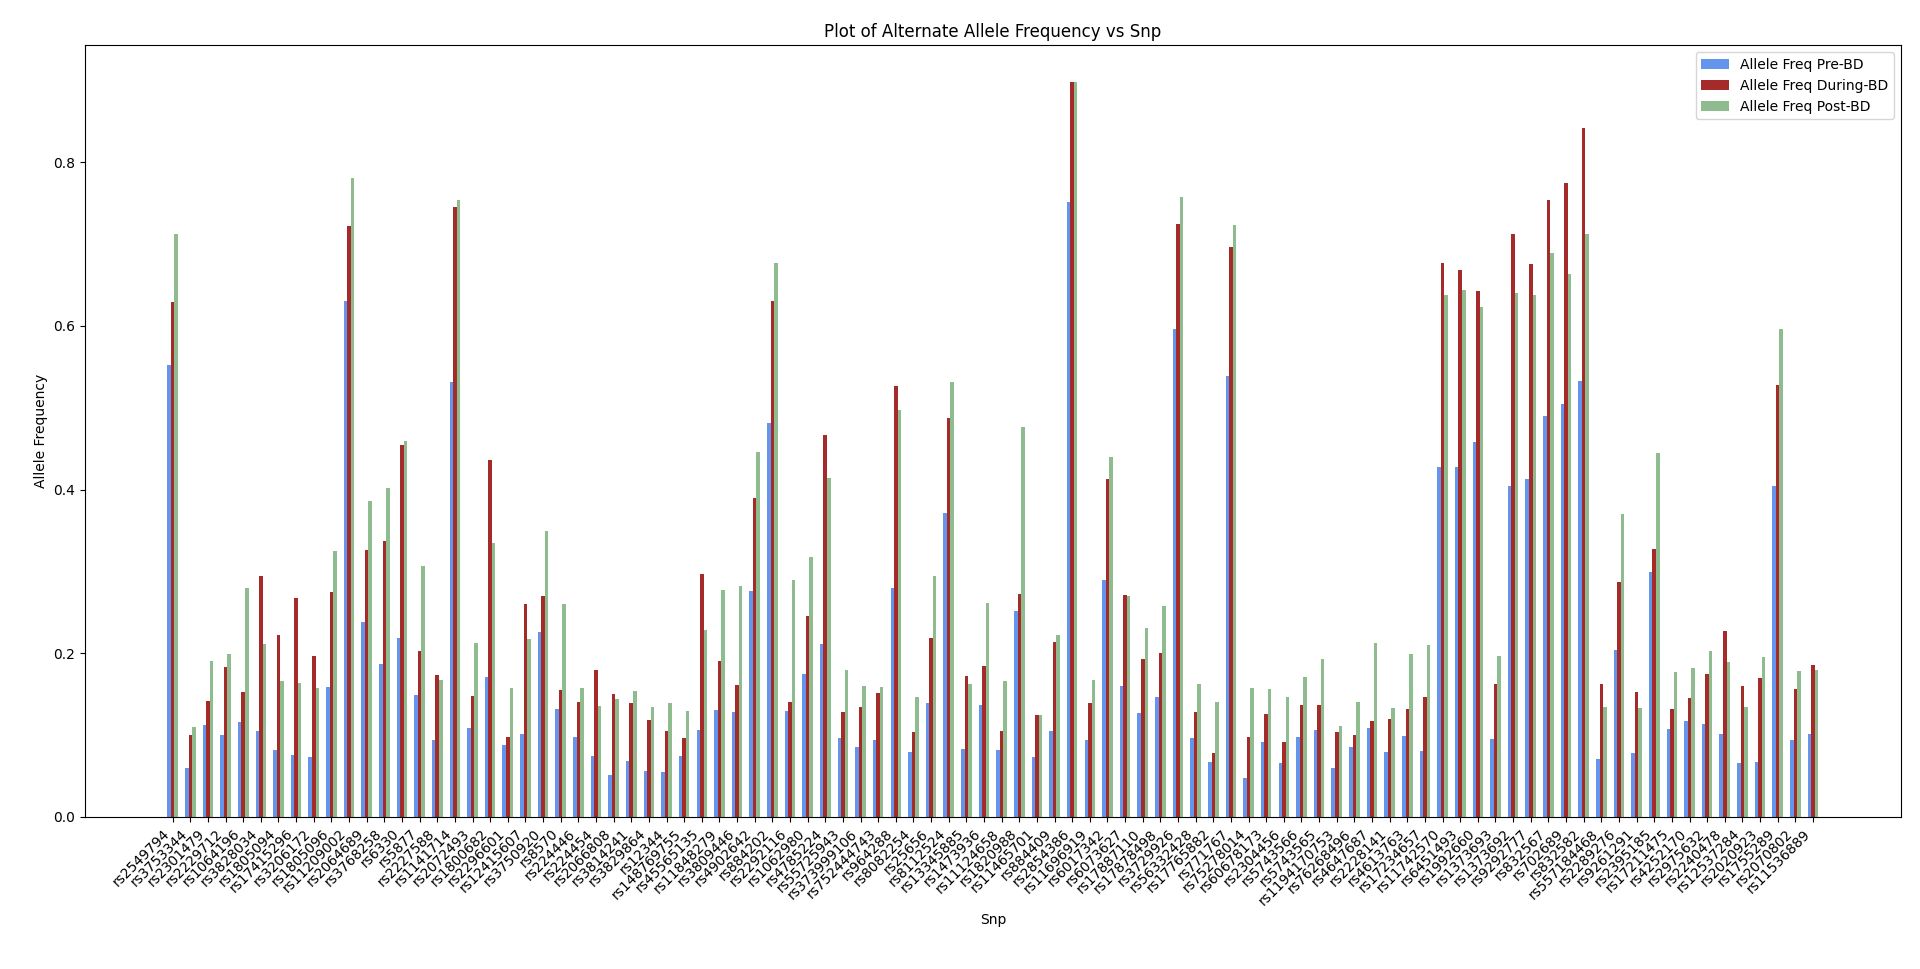
\includegraphics[width=0.7\textwidth]{images/snp-vs-allele-freq.png}
    \caption{Alternate Allele Frequencies vs SNPs}
  \end{figure}

\subsection{Fixation Index Analysis}
After using the values from the above plots, we can create a graph of FST values vs relevant SNPs. The fixation index is a representation of how diverse and differentiated that allele is in the population. Our research included the fixation index of London in two time periods: before-during London and during-after London (with the main event being the Black Death in the 1400s). The plot of the FST index values only included data of SNP’s where the after-during Black Death values for FST were higher than the before-during time period. These were then plotted on a plot with FST values on the y-axis and SNPs on the x-axis.


  \begin{figure}
  \centering
    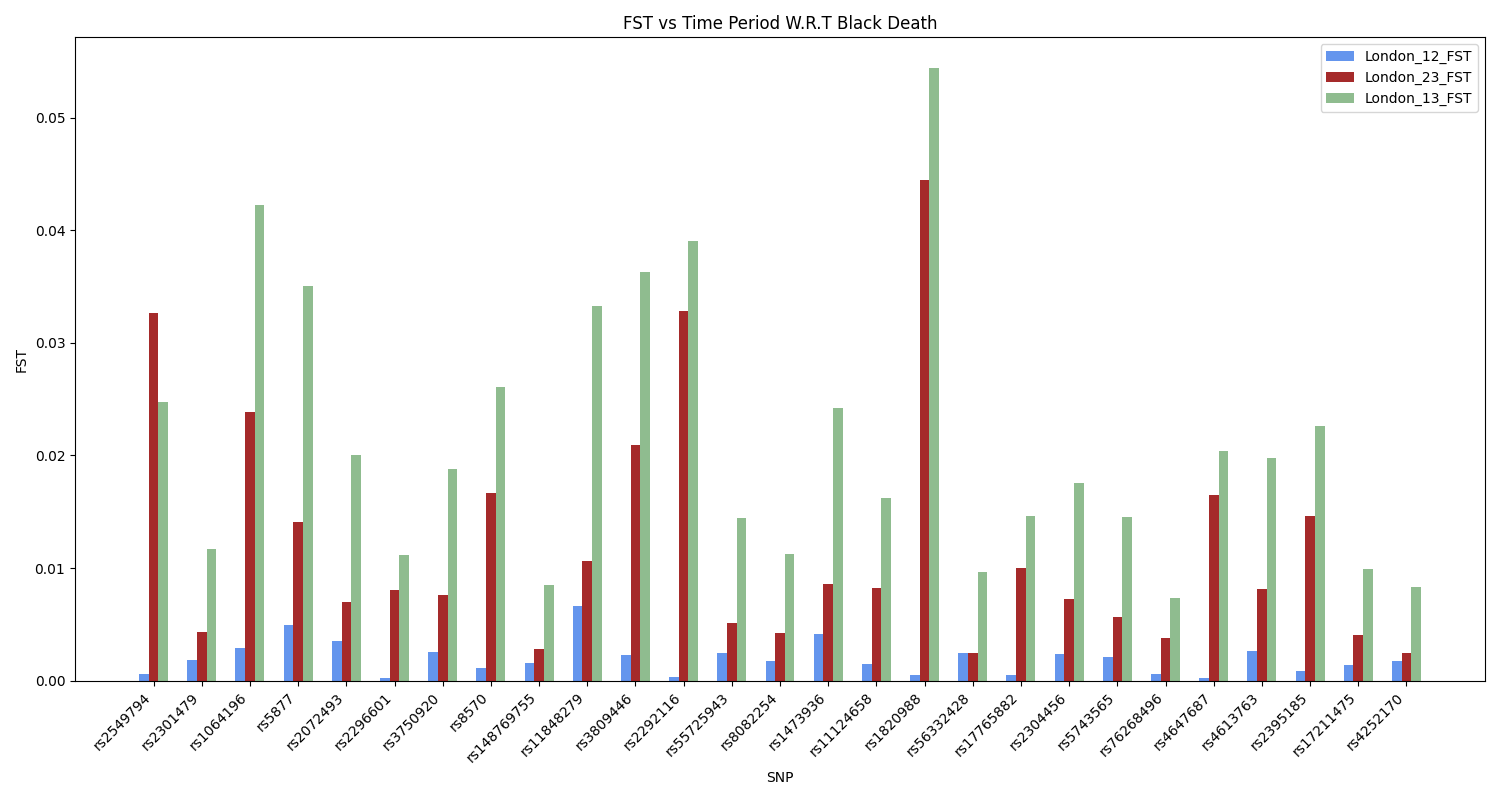
\includegraphics[width=0.7\textwidth]{images/snp-vs-fst.png}
    \caption{Alternate Allele Frequencies vs SNPs}
  \end{figure}

\subsection{ERAP2 and \textit{Y. Pestis} Stimulation}
Finall, computations methods were used to create a boxplot of cytokine values which were plotted against the three types of genotypes of the rs2549794 SNP. However, to actually compare the role of the Y. Pestis to the cytokine value, a non-infected sample was also used to create. The plot of Cytokine values vs genotypes (infected and non-infected) are shown in Figure 3.

  \begin{figure}
  \centering
    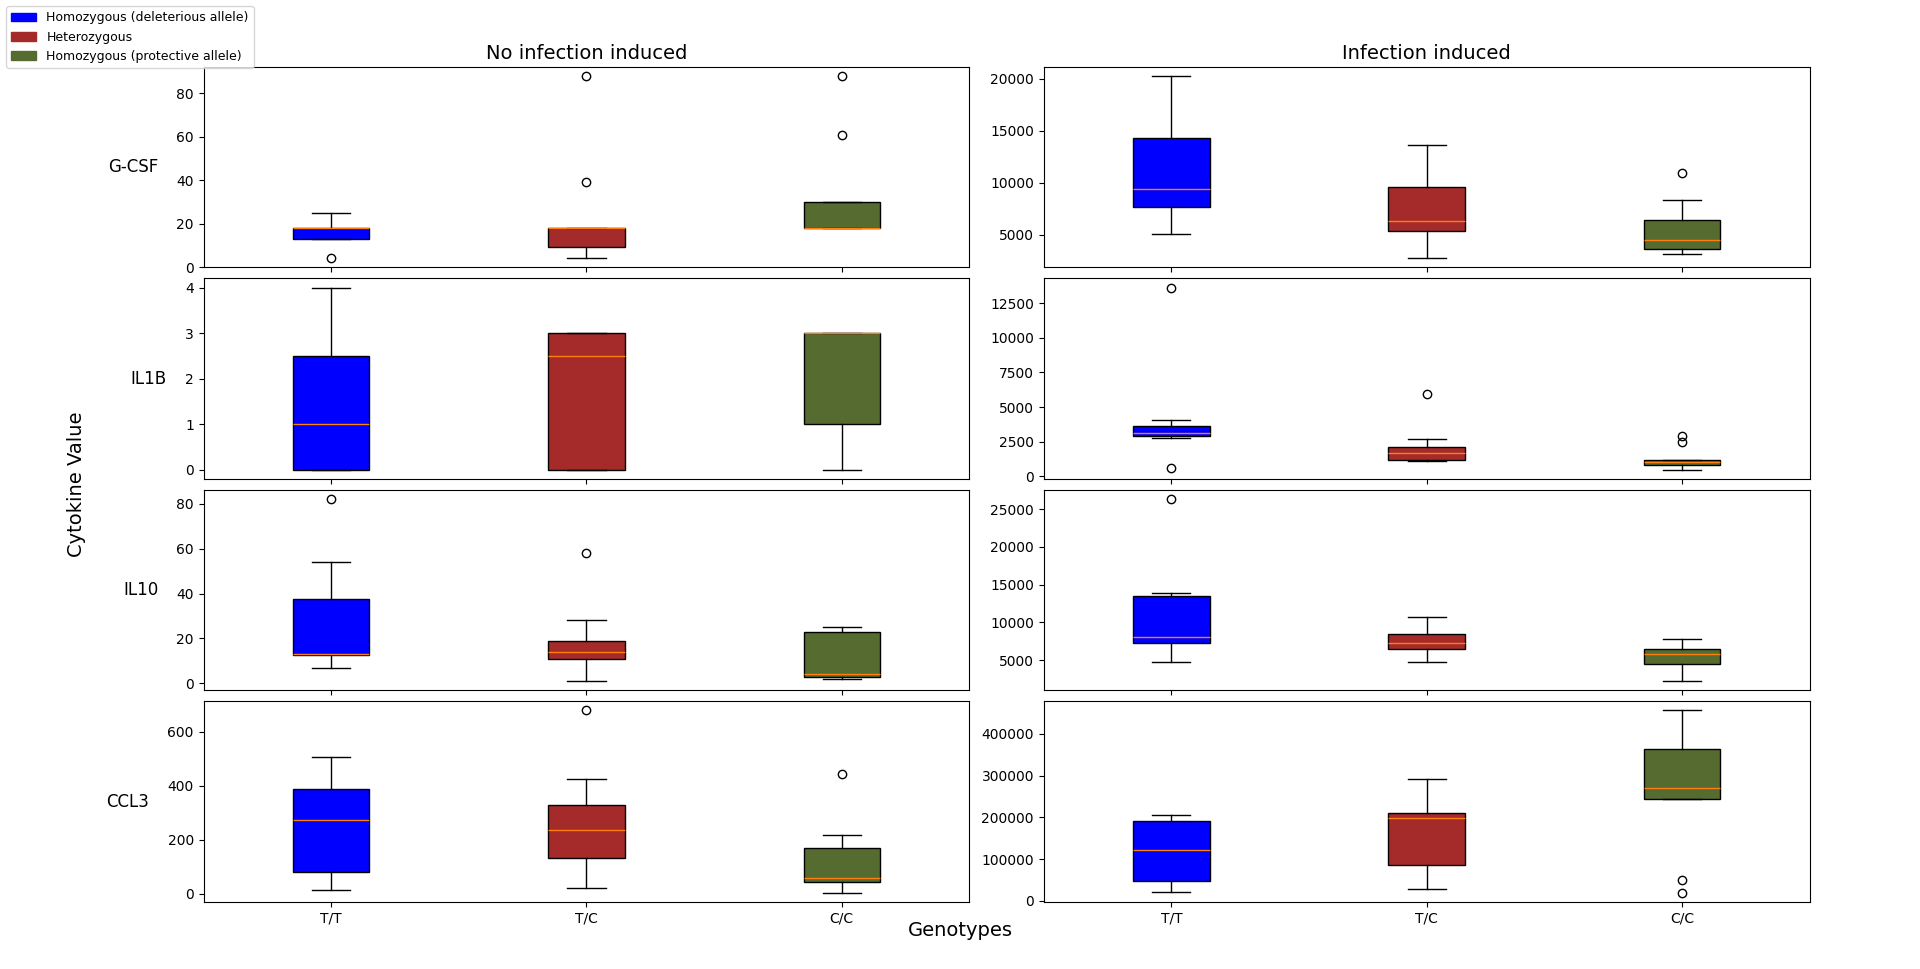
\includegraphics[width=0.7\textwidth]{images/boxplot.png}
    \caption{Alternate Allele Frequencies vs SNPs}
  \end{figure}

\section{Implications}
From the alternate allele frequencies vs SNP plot (Figure 1), the trend can be observed that amongst the important SNPs, the pre Black Death frequencies are much lower than post or during Black Death frequencies. This implies that there was definitely an alteration by the bacteria Yersinia. Pestis, caused the finding of increased alternate allele frequency within that SNP. However, to get more conclusive evidence that the allele, broadly the ERAP2 gene, has actually been altered, the FST index data has to be analyzed in the context of the bacteria and its effect on the particular gene and population.

The fixation index (Figure 2) shows how much the alternate allele, the allele hypothesized as offering selective immunity, is differentiated or prevalent in the population of London before, during and after the Black Death. From the plot, we can see that the rs2549794 SNP has a huge increase in distribution of the alternate allele after the black death. However, before the black death, the presence was almost non-existent. From all the plots, it was the only one that had such a drastic increase in distribution of alternate alleles, hinting that it underwent the most genetic change amongst genes associated with the immune system.

Finally, to completely finish the association studies that we’re running, it is vital to include how certain genotypes of the SNP in the ERAP2 gene responded to stimulation under the Y. Pesits bacteria. However, the dataset includes some outliers in the forms of association to pathogen influence, and we wouldn’t want to study cytokines that don’t associate themselves when under attack by pathogens. Hence, From Figure 3, a basic conclusion can be reached that exposure to pathogens to the like of Y. Pestis increases the production of cytokine response levels or values in four types of cytokines: G-CSF, IL1B, IL10, and CCL3. All except the CCL3 cytokine are pro-inflammation, meaning that they defend against the pathogens by creating inflammation-like conditions. Hence, the output will make sense since the cytokine is trying to fend off the bacteria. 

Further, an indirect connection can be made to inducing autoimmune disorders. Prolonged exposure to such bacteria can lead to the creation of autoimmune conditions, even though they offer immunity to the host organism. Moreover, the people who survived usually do so because of the presence of that protective allele in the body of that organism. 
 
\section{Future Work}
There is a wide range of extensions to this project that can massively benefit both the project and the historic epidemiologic. Firstly, this project highlights the need for more in-depth genomic analysis and techniques. It is important because the ancient data available is mostly available for the European population. 

Developing models that predict the future burden of autoimmune disorders and infectious diseases based on genetic susceptibility data. This can help healthcare systems plan and allocate resources more efficiently. Further, the development of preventive health strategies, such as genetic counseling and early intervention programs, to mitigate the risk of genetic predispositions manifesting as diseases.
Understanding genetic susceptibility can help in designing vaccines that are more effective for individuals with certain genetic profiles. Personalized vaccines could improve immunity in populations that are genetically predisposed to certain infections.


\section{References}‌
\bibliographystyle{plain}
\bibliography{references}

Klunk, Jennifer, et al. “Evolution of Immune Genes Is Associated with the Black Death.” Nature, vol. 611, no. 7935, Nature Portfolio, Oct. 2022, pp. 312–19, https://doi.org/10.1038/s41586-022-05349-x. Accessed 2 Aug. 2024.
\end{document}